%%%%%%%%%%%%%%%%%%%%%%%%%%%%%%%%%%%%%%%%%%%%%%%%%%%%
\section{Informed Plan Selection}\label{sec:coverage}
%%%%%%%%%%%%%%%%%%%%%%%%%%%%%%%%%%%%%%%%%%%%%%%%%%%%

The first part of this paper addresses the task of determining when decisions along the active execution trace may be considered \textit{informed enough} for outcomes to be included as learnable instances for each \dt in that trace. For this we contrast two schemes, \CL\ and \BUL\ - and show that the conservative \BUL\ approach delivers more robust performance than the simpler \CL\ approach for the cases considered. For both approaches, the same probabilistic function $E$ (or exploration strategy) was used to make the plan selection at each junction of the active execution trace.

In subsequent work we keep the \CL\ and \BUL\ recording methods constant, and adjust the probabilistic plan selection function $E$ to evaluate the impact on the learning outcome. Motivated by the polarity between the two approaches, we consider if an informed probabilistic selection function $E'$ may be constructed to yield a \textit{middle ground} approach that applies better in the general case. This would be valuable since if a \CL+$E'$-based approach yields comparable performance to any \BUL+$E^*$-based approach, then the former is preferred as \CL\ is much simpler than \BUL. Interestingly we find that such a formulation is possible and that an informed exploration strategy that leverages both the domain knowledge (inherent in the goal-plan tree hierarchy) as well as the ongoing learning (agent's experience so far) can combine the benefits of both \CL\ and \BUL.

We start by quantifying the quality of (or our \textit{confidence} in) the hypotheses of a \dt for a unknown but learnable subspace $S$ of worlds $[W_1 \ldots W_n]$. At the beginning of a run we have no learnable instances and for a given goal-plan tree node $T$ our probability of success $p_T(W)$ in world $W \in S$ is given by the default probability $P_d=0.5$. After the first instance is recorded, the \dt will generalise the result to the full space of $S$ (i.e. $\forall W \in S$) leading to likely \textit{misclassification}. Intuitively we know that as more and more $W \in S$ are witnessed and recorded, the \dt's classification over $S$ will improve. Our two approaches may be described in terms of confidence as follows: \CL\ always assumes full confidence in the \dt but suffers from misclassification errors (that are eventually rectified through subsequent learning from misinformed choices); \BUL\ uses the static $\epsilon$ and $k$ values to determine the boundary for our confidence in the \dt (with the trade-off that for the period of no confidence the best we can do is use $P_d$).

One way to improve this situation is to instead compute a smooth transition from zero-confidence in the \dt classification to full-confidence, based on experience. We identify two orthogonal properties, \textit{choices} and \textit{subspace} that are integral to informed decision making by the learning nodes in our agent. Choices refer to the set of all statically computable execution paths \textit{below} a goal node in the goal-plan tree hierarchy. Subspace refers to the set of all worlds that are learnable for the \dt at that node. Defined in those terms, we label a \dt \textit{not informed} if no choices have been recorded in any world of the subspace, or \textit{fully informed} when all choices have been covered in every world of the subspace. In fact, we can construct a measure of our confidence in the \dt based on the degree of \textit{coverage} of all choices in all subspace associated worlds.

\begin{equation}
\label{eqn:coverage}   
E': p'_T(W)= P_d + \left[  c_T(S) *  \left( p_T(W) - P_d \right)  \right]
\end{equation}

Equation \ref{eqn:coverage} shows how a confidence measure based on coverage may be used to modify the final plan selection probability. The idea is to bias the \dt classification (probability of success) of world $W$ in node $T$ given by $p_T(W) \in [0 \ldots 1]$ with the coverage $c_T(S) \in [0 \ldots 1]$ of subspace $S$ given $W \in S$. Initially the coverage is zero, so the revised probability $p'_T(W) = P_d$ the default probability of success. As coverage $\rightarrow 1$, the revised probability $p'_T(W) \rightarrow p_T(W)$ the \dt classification. This gives a progressive transition to the \dt classification as more experience is acquired (Figure \ref{fig:coverage-surface}).

\begin{figure}[ht]
   \centering
   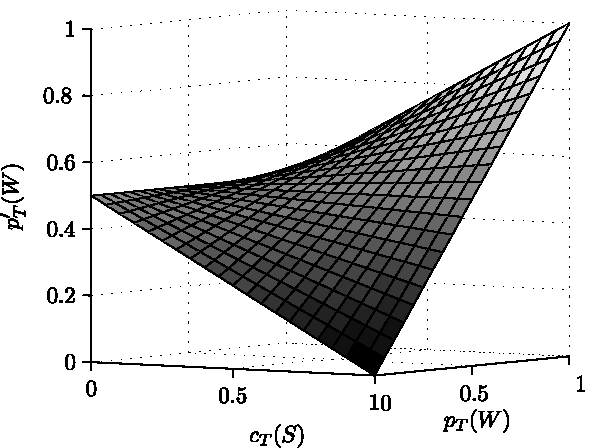
\includegraphics[width=\columnwidth]{figs/coverage-surface}
   \caption{How confidence (coverage) is used to adjust \dt classification for plan selection.}
   \label{fig:coverage-surface}
\end{figure}


The coverage $c_T(S)$ itself is calculated and stored each time a result is recorded for node $T$. The calculation is performed in turn for each node in the active execution trace starting at the leaf node where the failure occurred, and the coverage is updated progressively up the tree hierarchy. Full coverage at a node $T$ has a computation cost of $C(T)*|S|$ where $C(T)$ is the total number of choices below $T$ and $|S|$ is the number of worlds in the subspace. Practically however, it costs significantly less since choices below $T$ are effectively AND/OR trees, and each time an AND node fails the subsequent nodes are not tried and are assumed covered for that world. The full memory cost for a subspace with $a$ boolean attributes is $2^a*C(T)$ however we only require $2^a$ for the implementation since we do not keep track of each individual path below $T$ but only how many distinct paths below $T$ have been tried in a given world. The only unknown in the coverage calculation is $S$ since we do not know upfront the subspace to be learnt. A fairly useful estimate of $c_T(S)$ for practical use can however be constructed by averaging the individual coverages $c_T(W_i)$ of all previously seen worlds at node $T$. 

\subsection{Results}

Given our base approaches \CL\ and \BUL, the original probabilistic plan selection function $E$, and the new coverage-based plan selection function $E'$ (Equation \ref{eqn:coverage}), we are able to run four different learning configurations: the earlier $+E$ configurations (\CL+$E$, \BUL+$E$) and the new $+E'$ configurations (\CL+$E'$, \BUL+$E'$).

For the \CL-favouring structure $\T_1$ we find that the new $+E'$ configurations perform equally well to the original $+E$ configurations, so while there is no significant improvement in either \CL\ or \BUL, there is also no loss in performance. Similarly, for the typical structure $\T_3$ where both \CL\ and \BUL\ perform equally well, the choice of $E*$ has no significant impact. For $\T_1$ and $\T_3$ then, the $+E'$ results are the same as those reported for the original $+E$ configurations in Figure \ref{fig:T1_result} and Figure \ref{fig:T3_result}.

The impact of $E'$ is apparent in $\T_2$ however, a structure that favours the conservative \BUL\ approach (Figure \ref{fig:T2_result}). While \BUL\ shows similar performance in this case irrespective of the choice of $E^*$, \CL\ however is dramatically improved as a result of $E'$. Figure \ref{fig:T2_result2} shows this change with the new $+E'$ configurations (diamonds for \BUL\ and squares for \CL) superimposed over the original $+E$ results of Figure \ref{fig:T2_result} (circles for \BUL\ and triangles for \CL). So for the \BUL-favouring structure $\T_2$, the \CL+$E'$ (squares) approach is now much closer to \BUL+$E^*$ performance than the previous \CL+$E$ (triangles) approach.

\begin{figure}[ht]
\centering
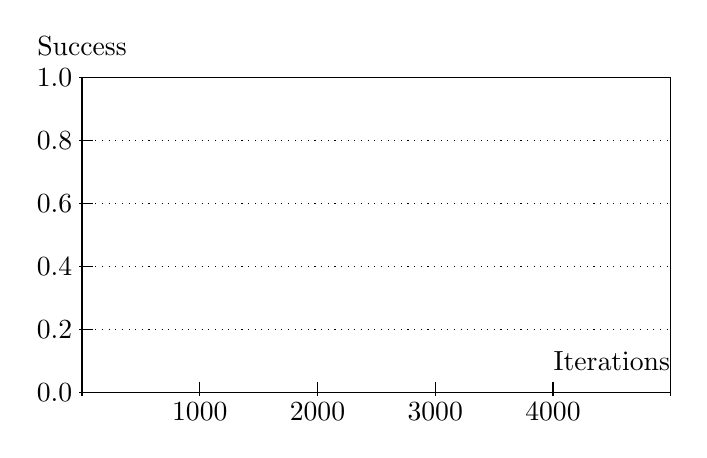
\begin{tikzpicture}[x=0.0015cm,y=4cm]
    % Draw the axes and grid lines
    \draw[-] (0,0) -- (0,1) -- (5000,1) -- (5000,0) -- cycle; 
    \draw[-,thin, dotted, ystep=0.2, xstep=5000] (0,0) grid (5000,1);
    \foreach \x in {0,1000,...,5000}  \draw [-,xshift=0](\x,4pt) -- (\x,-1pt);
    \foreach \y in {0.0,0.2,0.4,0.6,0.8,1.0}  \draw [-,yshift=0](4pt,\y) -- (-1pt,\y);
    \foreach \x/\xtext in {1000/1000, 2000/2000, 3000/3000, 4000/4000} \node at (\x,0) [below] {$\xtext$};
    \foreach \y/\ytext in {0.0,0.2,0.4,0.6,0.8,1.0}  \node at (0,\y) [left] {$\ytext$};
    \node at (0,1.1) {Success};
    \node at (4500,0.1) {Iterations};
    \draw[-] plot[mark=square,mark size=2,mark options={color=black}] 
			file {data/test05v5gm.CC.tikzdata};
    \draw[-,thin,densely dashed,gray] plot[mark=triangle,gray,mark size=3,mark options={color=gray}] 
			file {data/test05v5gm.CP.tikzdata};
    \draw[-] plot[mark=diamond,mark size=3,mark options={color=black}] 
			file {data/test05v5gm.SC.tikzdata};
    \draw[-,thin,densely dashed,gray] plot[mark=o,gray,mark size=2,mark options={color=gray}] 
			file {data/test05v5gm.SP.tikzdata};

\end{tikzpicture}
\caption{Comparison of the new configurations \BUL+$E'$ (diamonds) and \CL+$E'$ (squares) against the earlier \BUL+$E$ (circles) and \CL+$E$ (triangles) for the \BUL-favouring structure $\T_2$.}
\label{fig:T2_result2}
\end{figure}

We now consider a new structure $\T_4$ that is based on the typical setting (so is not intentionally biased towards one approach), and that has the property that a world $W$ may have two solutions, each in a different sub-tree. Furthermore one solution is always \textit{better} than the other because it has a higher chance of success (in our environment we model this by varying the number of actions required in the solution where each action has a $10\%$ chance of failure). Finally, the structure is crafted so that the likelihood of finding the sub-optimal solution is higher. The purpose is to understand how our approaches behave when optimality is important. Here we expect that the coverage-based exploration of $E'$ should benefit over $E$ in finding the optimal solutions first. 

\begin{figure}[ht]
\centering
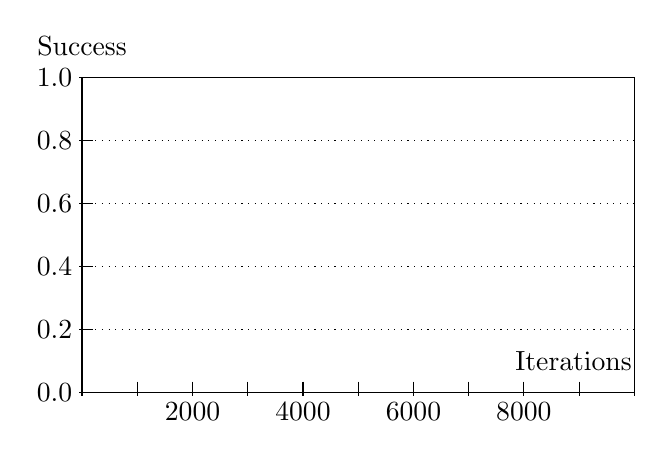
\begin{tikzpicture}[x=0.0007cm,y=4cm]
    % Draw the axes and grid lines
    \draw[-] (0,0) -- (0,1) -- (10000,1) -- (10000,0) -- cycle; 
    \draw[-,thin, dotted, ystep=0.2, xstep=10000] (0,0) grid (10000,1);
    \foreach \x in {0,1000,...,10000}  \draw [-,xshift=0](\x,4pt) -- (\x,-1pt);
    \foreach \y in {0.0,0.2,0.4,0.6,0.8,1.0}  \draw [-,yshift=0](4pt,\y) -- (-1pt,\y);
    \foreach \x/\xtext in {2000/2000, 4000/4000, 6000/6000, 8000/8000} \node at (\x,0) [below] {$\xtext$};
    \foreach \y/\ytext in {0.0,0.2,0.4,0.6,0.8,1.0}  \node at (0,\y) [left] {$\ytext$};
    \node at (0,1.1) {Success};
    \node at (8900,0.1) {Iterations};
    \draw[-] plot[mark=square,mark size=2,mark options={color=black}] 
			file {data/testMultiSolutionsR.CC.tikzdata};
    \draw[-,thin,densely dashed,gray] plot[mark=triangle,gray,mark size=3,mark options={color=gray}] 
			file {data/testMultiSolutionsR.CP.tikzdata};
    \draw[-] plot[mark=diamond,mark size=3,mark options={color=black}] 
			file {data/testMultiSolutionsR.SC.tikzdata};
    \draw[-,thin,densely dashed,gray] plot[mark=o,gray,mark size=2,mark options={color=gray}] 
			file {data/testMultiSolutionsR.SP.tikzdata};

\end{tikzpicture}
\caption{Comparison of all configurations (\BUL+$E'$ (diamonds), \CL+$E'$ (squares), \BUL+$E$ (circles), \CL+$E$ (triangles)) for new structure $\T_4$ with local solutions.}
\label{fig:T4_result}
\end{figure}

Figure \ref{fig:T4_result} shows the results for $\T_4$ where \CL+$E'$ (squares) easily outperforms all other configurations. The reason why the $+E$ configurations (circles and triangles) are sub-optimal is because they do not take into account the structure of the tree and therefore tend to focus exploration in the sub-tree where the first solution was found (which likely is the sub-optimal one in our case). 

Note that \BUL+$E'$ (diamonds) does not perform well in $\T_4$ even though it is coverage-based and does consider the tree structure. In fact, an interesting observation during our extensive testing with several different tree structures is that \BUL+$E'$ always show similar performance to \BUL+$E$. This is because the $\StableGoal(G,w,k,\epsilon)$ check of \BUL\ inherently results in close to full coverage, effectively reducing $p'_T(W)$ to $p_T(W)$ in Equation \ref{eqn:coverage}. This means that for \BUL\, the $E$ and $E'$ selection functions are effectively the same.

The above results are significant because they highlight a configuration \CL+$E'$ that performs well in \textit{all} proposed structures: the \CL-favouring $\T_1$, the \BUL-favouring $\T_2$, the typical setting $\T_3$, and the typical setting with optimal solutions $\T_4$, making it a good candidate for the general setting. Moreover, the \CL-based configuration is a simpler alternative to the \BUL-based configuration, further adding to it's appeal.


\subsection{Discussion}

In Section \ref{sec:coverage} we presented a \textit{coverage}-based confidence measure that combined with the \dt classification gives an informed plan selection function (Equation \ref{eqn:coverage}) that benefits our context learning approaches \CL\ and \BUL. Now, since the coverage $c_T(S)$ in Equation \ref{eqn:coverage} is simply a confidence measure, then the way it is \textit{used} will determine the weighting of the confidence towards the final plan selection probability $p'_T(W)$. For instance we could replace $c_T(S)$ in Equation \ref{eqn:coverage} with $c_T(S)^{1/b}$ where $b$ is the weighting (and $b=1$ gives us the original Equation \ref{eqn:coverage}). Then adjusting $b \rightarrow 0, (0 \ne b < 1$) we get more \BUL+$E$-like performance, while adjusting $b \rightarrow \infty (b > 1)$ will result in more \CL+$E$-like performance. In fact, an improved agent could reference the (static) goal-plan tree structure at runtime and adjust $b$ automatically based on the offline compiled knowledge of which approach works better for which tree topology. This extension is left as a future implementation exercise.

We noted earlier in Section \ref{sec:experiments} that plan execution in real systems is often not cost-free, so presumably the agent would not execute a plan with too low a probability of success. We also show that such deliberation does not favour \CL\ but does \BUL. It is clear that choosing not to execute a plan below a threshold probability of failure would also hurt the candidate \CL+$E'$ configuration (though not as much as \CL+$E$). For such systems, we suggest that the weighting $b$ be used to get the preferred \BUL-like performance.

One critique of the coverage-based confidence measure is that it has a defined start ($c_T(S)=0$) and end state ($c_T(S)=1$). For a real system however, learning and re-learning will occur in an endless loop as the agent continually tries to adapt to a changing environment. This implies that our confidence in a \dt's classification would also require calibration based on a changing environment. If the change in the environment is deliberate (for instance the agent was moved into a new environment) then the coverage $c_T(S)$ could be reset and confidence \textit{re-built}. Without such a signal the agent must rely of measuring per-goal performance in order to pick up failures that could be attributed to environmental changes. The problem of identifying changes that warrant new learning as compared to adapting previous learning, however, is generally considered to be a much harder one.

